\documentclass[border=12pt]{standalone}
\def\pgfsysdriver{pgfsys-dvisvgm.def}
\usepackage[dvisvgm]{xcolor}
\usepackage{xeCJK}
\setCJKmainfont{HaranoAjiGothic-Regular.otf}[BoldFont=HaranoAjiGothic-Bold.otf]
\setCJKsansfont{HaranoAjiGothic-Regular.otf}[BoldFont=HaranoAjiGothic-Bold.otf]
\usepackage{amsmath,amssymb,tikz,lmodern}
\usetikzlibrary{arrows.meta,positioning,calc,fit,backgrounds}
\renewcommand{\familydefault}{\sfdefault}
\definecolor{ink}{HTML}{25322F}
\definecolor{green}{HTML}{246657}
\definecolor{tint}{HTML}{EEF4F0}
\definecolor{soft}{HTML}{C6D2CC}
\definecolor{muted}{HTML}{52615B}
\newif\ifJapanese
\newcommand{\Tx}[2]{\ifJapanese #1\else #2\fi}
\newcommand{\Eff}{\overline{\operatorname{Eff}}}
\newcommand{\heading}[3]{{\color{green}\bfseries #1\quad\Tx{#2}{#3}}\\[5pt]}
% A white rectangle makes the complete citation label clickable, including spaces.
\newcommand{\refurl}[2]{\special{dvisvgm:raw <a xlink:href="#1" target="_blank" rel="noopener noreferrer">}{\setlength{\fboxsep}{0pt}\colorbox{white}{\color{green}\underline{\strut #2}}}\special{dvisvgm:raw </a>}}
\newcommand{\refedge}[3]{\refurl{\csname source#1\endcsname\string##page=#2}{#3}}
\newcommand{\SF}[2]{\refedge{sf}{#1}{#2}}
% GitHub's file preview does not support PDF page fragments.
\newcommand{\LA}[2]{\refurl{\sourcela}{#2}}
\newcommand{\Sch}[2]{\refedge{sch}{#1}{#2}}
\newcommand{\PS}[2]{\refedge{ps}{#1}{#2}}
\tikzset{
 card/.style={draw=soft,fill=white,rounded corners=2pt,align=left,text=ink,font=\fontsize{10.5}{14}\selectfont,inner xsep=12pt,inner ysep=10pt,text width=14.4cm},
 half/.style={card,text width=6.45cm,minimum height=2.05cm},
 result/.style={card,draw=green,fill=tint,line width=.9pt},
 reason/.style={align=left,text=muted,font=\fontsize{9}{12}\selectfont,inner sep=0pt,text width=12.7cm},
 branchreason/.style={reason,text width=5.95cm},
 edge/.style={-{Stealth[length=2.4mm]},draw=green,line width=1pt},
 wire/.style={draw=green,line width=1pt},
}
% Keep the arrow in a dedicated left gutter; explanations never cover it.
\newcommand{\flow}[3]{
 \coordinate (#2-from) at ($(#1.south)+(-6.9,0)$);
 \coordinate (#2-to) at ($(#2.north)+(-6.9,0)$);
 \draw[edge] (#2-from)--(#2-to);
 \node[reason,anchor=west] (#2-reason) at ($(#2-from)!.5!(#2-to)+(.55,0)$) {#3};
}


\newcommand{\CiteSource}[2]{\refurl{\csname source#1\endcsname}{#2}}

\expandafter\def\csname sourceK4N\endcsname{https://github.com/openai/math/blob/adc7f1241b42e322a6451854ab7e4b4c146bf78a/preprints/Abundance-after-nonvanishing-for-compact-Kahler-fourfolds-September-27-2026/paper.pdf}
\expandafter\def\csname sourceHLL\endcsname{https://arxiv.org/pdf/2508.14634v2}
\expandafter\def\csname sourceDO\endcsname{https://arxiv.org/pdf/2306.00671v4}
\expandafter\def\csname sourceDHP\endcsname{https://arxiv.org/pdf/2205.12205v3}
\expandafter\def\csname sourceFT\endcsname{https://arxiv.org/pdf/2205.14801v7}
\expandafter\def\csname sourceSai\endcsname{https://arxiv.org/pdf/2204.09026v5}
\expandafter\def\csname sourceSS\endcsname{https://perso.pages.math.cnrs.fr/users/claude.sabbah/MHMProject/mhm_chap16.pdf}
\expandafter\def\csname sourceFG\endcsname{https://www.math.kyoto-u.ac.jp/~fujino/fg-comp-final.pdf}
\expandafter\def\csname sourceSL\endcsname{https://github.com/openai/math/blob/adc7f1241b42e322a6451854ab7e4b4c146bf78a/preprints/Lifting-sections-from-the-reduced-support-of-an-adjoint-September-27-2026/paper.pdf}
\expandafter\def\csname sourceLA\endcsname{https://github.com/openai/math/blob/adc7f1241b42e322a6451854ab7e4b4c146bf78a/preprints/Log-abundance-in-characteristic-zero-September-24-2026/paper.pdf}

\Japanesetrue
\begin{document}
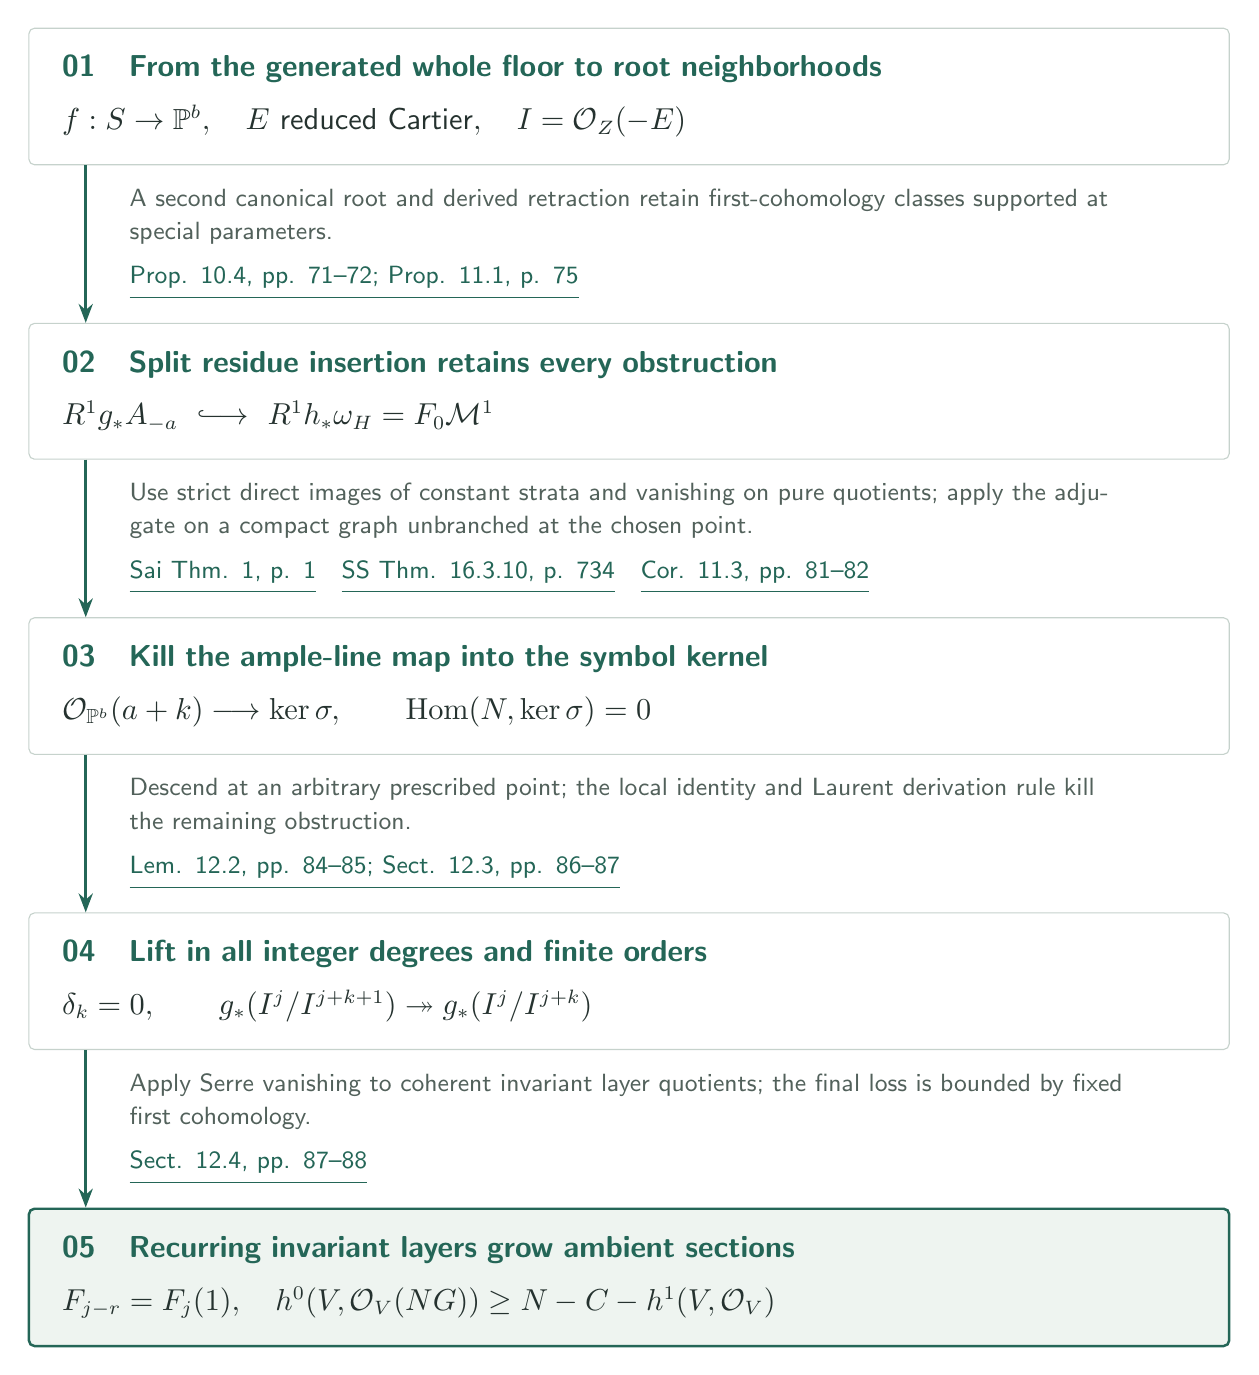
\begin{tikzpicture}
\node[card] (n0) {\heading{01}{生成された全floorからroot近傍へ}{From the generated whole floor to root neighborhoods}$f:S\to\mathbb P^b,\quad E\text{ reduced Cartier},\quad I=\mathcal O_Z(-E)$};
\node[card,below=2.0cm of n0] (n1) {\heading{02}{障害を失わないsplit residue挿入}{Split residue insertion retains every obstruction}$R^1g_*A_{-a}\ \lhook\joinrel\longrightarrow\ R^1h_*\omega_H=F_0\mathcal M^1$};
\flow{n0}{n1}{\Tx{第二のcanonical rootと導来retractionが、特殊パラメータに台を持つ第一cohomologyも保つ。}{A second canonical root and derived retraction retain first-cohomology classes supported at special parameters.}\\[4pt]\CiteSource{K4N}{Prop. 10.4, pp. 71--72; Prop. 11.1, p. 75}}
\node[card,below=2.0cm of n1] (n2) {\heading{03}{ample lineからsymbol kernelへの写像を消す}{Kill the ample-line map into the symbol kernel}$\mathcal O_{\mathbb P^b}(a+k)\longrightarrow\ker\sigma,\qquad\operatorname{Hom}(N,\ker\sigma)=0$};
\flow{n1}{n2}{\Tx{constant strataのstrict直像とpure商のvanishing。非分岐点を選ぶcompact graph上でadjugateを使う。}{Use strict direct images of constant strata and vanishing on pure quotients; apply the adjugate on a compact graph unbranched at the chosen point.}\\[4pt]\CiteSource{Sai}{Sai Thm. 1, p. 1}\quad \CiteSource{SS}{SS Thm. 16.3.10, p. 734}\quad \CiteSource{K4N}{Cor. 11.3, pp. 81--82}}
\node[card,below=2.0cm of n2] (n3) {\heading{04}{全整数次数・全有限次数で持ち上げ}{Lift in all integer degrees and finite orders}$\delta_k=0,\qquad g_*(I^j/I^{j+k+1})\twoheadrightarrow g_*(I^j/I^{j+k})$};
\flow{n2}{n3}{\Tx{任意の指定点へ降下し、局所恒等式とLaurent導分則で残る障害を消す。}{Descend at an arbitrary prescribed point; the local identity and Laurent derivation rule kill the remaining obstruction.}\\[4pt]\CiteSource{K4N}{Lem. 12.2, pp. 84--85; Sect. 12.3, pp. 86--87}}
\node[result,below=2.0cm of n3] (n4) {\heading{05}{不変層の反復から周囲の切断を増やす}{Recurring invariant layers grow ambient sections}$F_{j-r}=F_j(1),\quad h^0(V,\mathcal O_V(NG))\geq N-C-h^1(V,\mathcal O_V)$};
\flow{n3}{n4}{\Tx{巡回不変部分のcoherent層商にSerre vanishingを適用。最後の損失は固定の第一cohomology。}{Apply Serre vanishing to coherent invariant layer quotients; the final loss is bounded by fixed first cohomology.}\\[4pt]\CiteSource{K4N}{Sect. 12.4, pp. 87--88}}
\end{tikzpicture}
\end{document}
